\subsection{VQ-GAN + CLIP}
\begin{frame}[allowframebreaks]{VQ-GAN + CLIP}
    \large
    \textbf{VQ-GAN + CLIP} pairs two models so that vector quantization supplies the image generator and contrastive language-image pretraining supplies the text-based objective.

    \begin{itemize}
        \item \textbf{VQ-GAN:} A generative model that uses vector quantization to encode images into discrete latent codes, enabling efficient representation and high-quality image synthesis.
        \item \textbf{CLIP:} A model that learns visual representations by aligning images and text, allowing for zero-shot classification and improved understanding of visual content.
    \end{itemize}
\framebreak
    \textbf{How They Work Together:}
    \begin{itemize}
        \item \textbf{Image Generation:} VQ-GAN generates images by decoding quantized latent codes, while CLIP provides a text-based conditioning mechanism that guides the generation process.
        \item \textbf{Text Conditioning:} CLIP's text embeddings can be used to condition the VQ-GAN generator, allowing it to produce images that match specific textual descriptions.
        \item \textbf{Loss Function:} The similarity between generated image embeddings and text embeddings from CLIP can be used as a loss function to optimize the VQ-GAN generator, ensuring that the generated images align with the given text prompts.
    \end{itemize}
\framebreak
    \begin{figure}
        \centering
        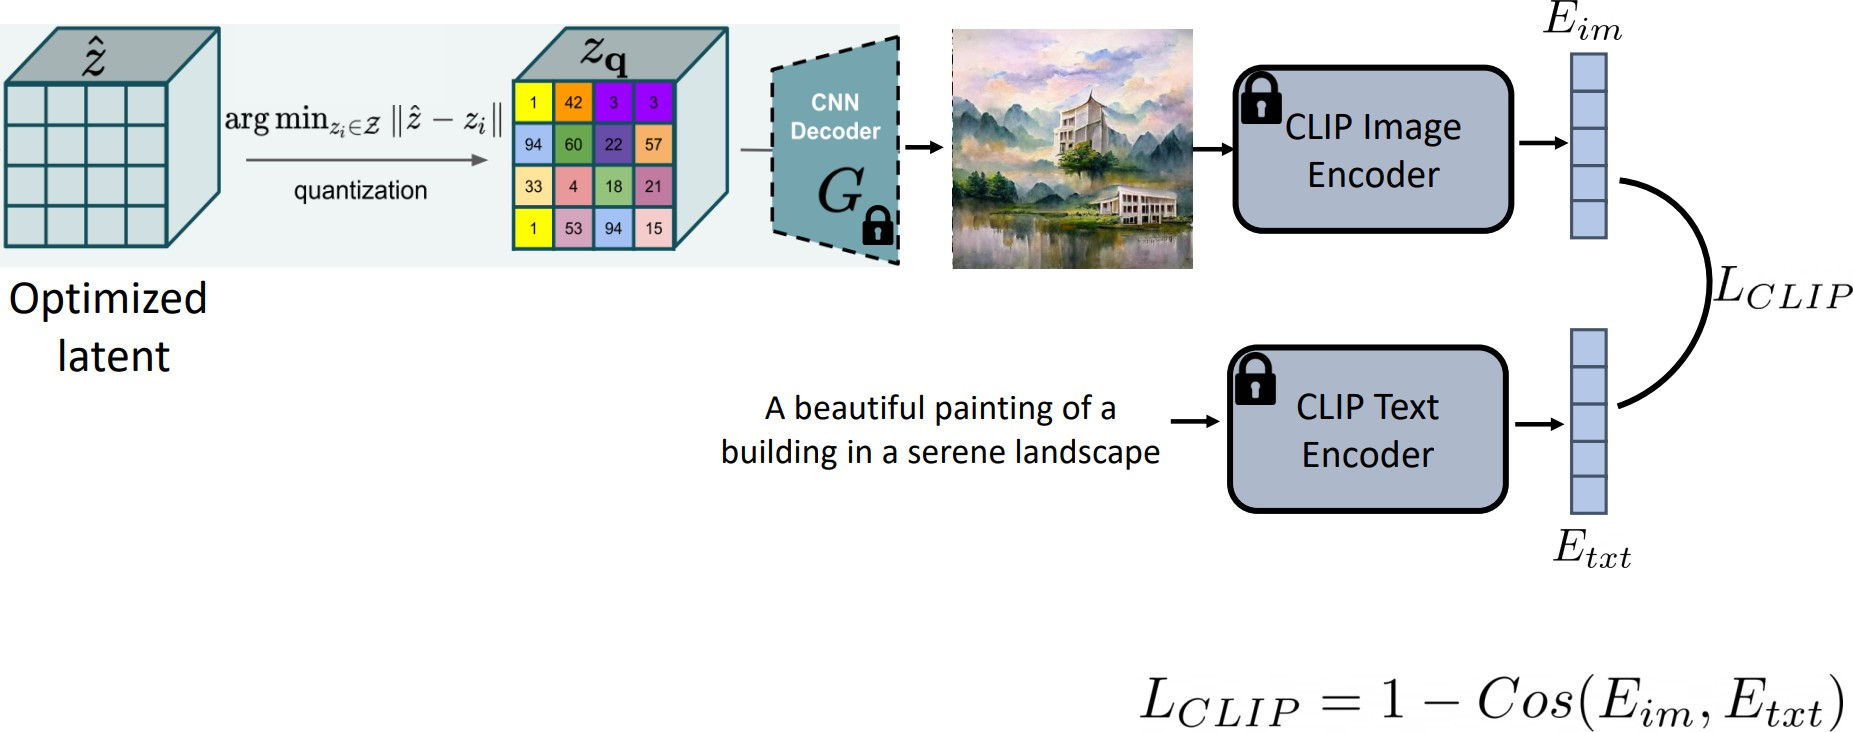
\includegraphics[width=1\textwidth,height=0.8\textheight,keepaspectratio]{images/video/slide_60_1_img.jpg}
    \end{figure}
    {\footnotesize{[VQGAN-CLIP: Open Domain Image Generation and Editing with Natural Language Guidance, Crowson et al., ECCV 2022]}}

\framebreak
    \large
    \textbf{Applications:}
    \begin{itemize}
        \item \textbf{Text-to-Image Synthesis:} VQ-GAN + CLIP can generate images based on textual descriptions, enabling creative applications like art generation and design.
        \item \textbf{Image Editing:} The combination allows for editing images based on text prompts, such as changing the style or content of an image while preserving its structure.
        \item \textbf{Zero-Shot Learning:} CLIP's zero-shot capabilities classify generated images into categories without additional training.
    \end{itemize}

\framebreak
    \begin{figure}
        \centering
        
\includegraphics[width=1\textwidth,height=0.85\textheight,keepaspectratio]{images/video/slide_61_1_img.png}
    \end{figure}
    {\footnotesize{[VQGAN-CLIP, Crowson et al., ECCV 2022, Fig.~2]}}
\end{frame}